\section{Implementation and Algorithms}
\label{sec:algs}
The implementation of this idea requires changing what information the \aivcalg algorithm uses to complete the proofs and generate MUSs. At each layer of analysis, the \aivcalg algorithm views the model as a constraint system consisting of the negation of the property in question (guarantees at lower levels, top-level properties at the highest level), and the supporting guarantees/assumptions from the direct child level. The information provided to this algorithm changes slightly when performing the minimal cut set algorithms.

\subsubsection{Implementation in Lustre}
In this approach, we use the all MIVCs algorithm and provide it a constraint system consisting of the negation of the top level safety property, the contracts of system components, as well as the faults in each layer constrained to false. It then collects the MUSs of this constraint system.

\begin{figure}[htbp]
	\hspace*{-2cm}
	\vspace{-0.1in} 
	\begin{center}
		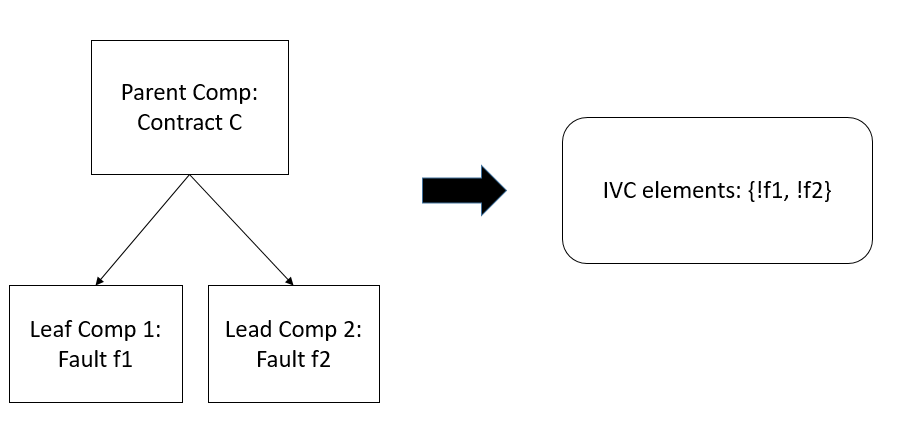
\includegraphics[scale=0.5]{images/ivcElements1.png}
	\caption{IVC Elements used for Consideration in a Leaf Layer of a System}
		\label{fig:ivcElements1}
	\end{center}
\end{figure}

Different layers of the architecture (and hence proof) provide slightly different information to the \aivcalg algorithm. This is ``given" to the IVC algorithm by the insertion of a Lustre statement with the keyword \texttt{\%IVC} followed by the fault activation literal. \\ \texttt{--\%IVC \_\_fault\_\_independently\_\_active\_\_sensor}\\

The constraints on that literal are given through the use of an assert statement in Lustre.\\ \texttt{assert (\_\_fault\_\_independently\_\_active\_\_sensor = false)}\\

The leaf nodes contribute only constrained faults to the IVC elements as shown in Figure~\ref{fig:ivcElements1}. In the non-leaf layers of the program, both contracts and constrained faults are considered as shown in Figure~\ref{fig:ivcElements2}. The reason for this is that the contracts are used to prove the properties at the next highest level and are necessary for the verification of the properties. The faults are used to provide safety pertinant information for the minimal cut sets. 

\begin{figure}[htbp]
	\hspace*{-2cm}
	\vspace{-0.1in} 
	\begin{center}
		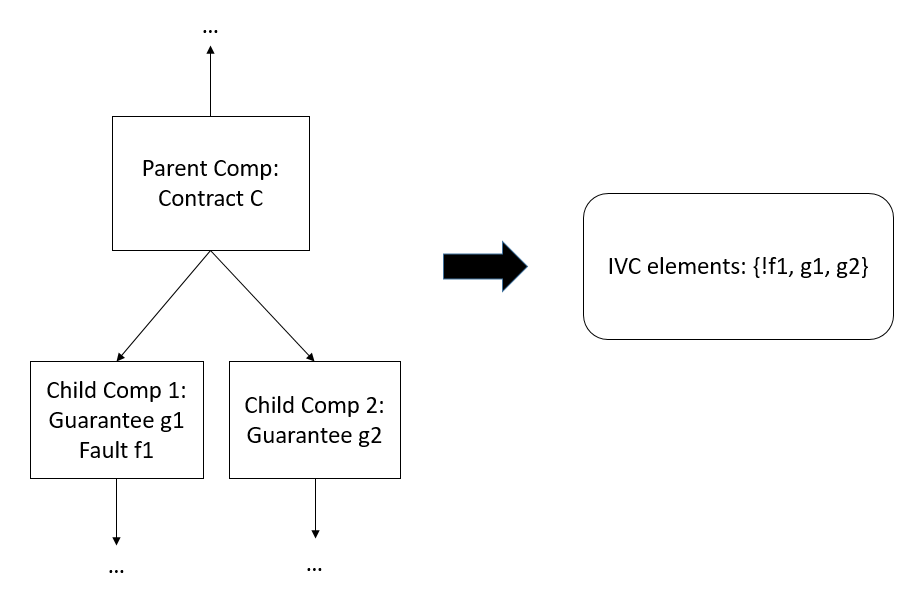
\includegraphics[scale=0.5]{images/ivcElements2.png}
	\caption{IVC Elements used for Consideration in a Middle Layer of a System}
		\label{fig:ivcElements2}
	\end{center}
\end{figure}

The all MIVCs algorithm returns the minimal set of these elements necessary to prove the properties. This equates to any contracts or inactive faults that must be present in order for the verification of properties in the model. From here, we perform a number of algorithms to transform all MIVCs into minimal cut sets.


%%%%%%%%%%%%%%%%%%%%%%%%%%%%%%%%%%%%%%%%%%%%%%%%%
%%%%%%%%%%%%%%%%%%%%            ALGORITHM DETAILS
\subsubsection{Algorithms}
The generation of \textit{MIVCs} traverses the program in a top down fashion. Likewise, the transformation of \textit{MIVCs} to MinCutSets traverses this program layer by layer if and only if all MIVCs have been generated. It is a requirement of the minimal hitting set algorithm that \textit{all} MUSs are used to find the MCSs~\cite{liffiton2016fast,gainer2017minimal,murakami2013efficient}. Thus, once all the MIVCs have been found and the minimal hitting set algorithm has completed, %our 
the MinCutSet Generation algorithm can begin. 

The MinCutSet Generation Algorithm begins with a list of MCSs specific to a top level property. These MCSs may contain a mixture of fault activation literals constrained to \textit{false} and %\textit{true} subcomponent contracts.
and subcomponent contracts constrained to \textit{true}. We remove all constraints from each MCS and call the resulting sets $I$, for \textit{Intermediate} set. Replacement of subcomponent contracts with their respective minimal cut sets can then proceed. For each of those contracts in $I$, we check to see if we have previously obtained a MinCutSet for that contract. If so, replacement is performed. If not, we recursively call this algorithm to obtain the list of all MinCutSets associated with this subcomponent contract. At a certain point, there will be no more contracts in the set $I$ in which case we have a minimal cut set for the current property. When this set is obtained, we store it in a lookup table keyed by the given property that this $I$ is associated with. 

A small example will illustrate this process. \danielle{Do I want to have a more concrete example? If so, pull from thesis proposal sensor example. If a shorter more abstract example is okay, do that.}







Algorithm~\ref{alg:generation_alg} describes this process.


\begin{algorithm}[htbp]
\SetKwFunction{FMain}{replace}
 \SetKwProg{Fn}{Function}{:}{}

	\Fn{\FMain{$P$}}{
		$List(I)$:= $List(MCS)$ for $P$ with all constraints removed \;
		\For{all $I \in List(I)$}{
			\eIf{there exists contracts $g \in I$}{
				\For{all constrained contracts $g \in I$}{
					\eIf{there exists $MinCutSets$ for $g$ in lookup table}{
						\For{all $minCut(g)$}{
							$I_{repl} = I$ \;
							$I_{repl} :=$ replace $g$ with $minCut(g)$ \;
							add $I_{repl}$ to $List(I)$ \;
						} %end for all cut sets of g
					}{
						replace($g$) \;
					} % end else if no cut sets in lookup table
				} % end for all constrained contracts in I
			}{
				add $I$ as $minCut(g)$ for $P$ \;
			} %end else if there exists contracts in I
		}%end for all I in list(I)
	}
%	\caption{Minimal Cut Set Generation Algorithm}
	\caption{MinCutSets Generation Algorithm}
	\label{alg:generation_alg}
\end{algorithm}

The number of replacements $R$ that are made in this algorithm are constrained by the number of minimal cut sets there are 
for all $\alpha$ contracts within the initial MCS. 

We call the set of all minimal cut sets for a contract $g$: $Cut(g)$. The following formula defines an upper bound on the number of replacements. The validity of this statement follows directly from the general multiplicative combinatorial principle. The number of replacements $R$ is bounded by the following formula:
\begin{equation}
\label{eq:bound}
  R \leq {\displaystyle \sum_{i=1}^{\alpha} }({\displaystyle \prod_{j=1}^{i} |Cut(g_j)|})  
\end{equation}


It is also important to note that the cardinality of $List(I)$ is bounded, i.e. the algorithm terminates. Every new $I$ that is generated through some replacement of a contract with its minimal cut set is added to $List(I)$ in order to continue the replacement process for all contracts in $I$. Adding to this set requires proof regarding termination.
\begin{theorem}
Algorithm~\ref{alg:generation_alg} terminates
\begin{proof}
No infinite sets are generated by the \aivcalg or minimal hitting set algorithms~\cite{Ghassabani2017EfficientGO,murakami2013efficient}; therefore, every MCS produced is finite. Thus, every $MinCutSet$ of every contract $g$ is finite. Furthermore, a bound exists on the number of additional intermediate sets $I$ that are added to $List(I)$: \\
$|List(I)| \leq R$ (Equation~\ref{eq:bound}).
\end{proof}
\end{theorem}

The reason for this upper bound is that for a contract $g_1$ in MCS, we make $|Cut(g_1)|$ replacements and add the resulting lists to $List(I)$. Then we move to the next contract $g_2$ in $I$. We must additionally make $|Cut(g_1)| \times |Cut(g_2)|$ replacements and add all of these resulting lists to $List(I)$, and so on throughout all contracts. Through the use of basic combinatorial principles, we end with the above formula for the upper bound on the number of additional intermediate sets.


\subsubsection{Pruning to Address Scalability}
The MinCutSets are filtered during this process based on a fault hypothesis given before analysis begins. The Safety Annex provides the capability to specify a type of verification in what is called a \textit{fault hypothesis statement}. These come in two forms: maximum number of faults or probabilistic analysis. Algorithm~\ref{alg:generation_alg} is the general approach, but the implementation changes slightly depending on which form of analysis is being performed. This pruning improves performance and diminishes the problem of combinatorial explosions in the size of minimal cut sets for larger models. \\

\textbf{Max $N$ Analysis Pruning} This statement restricts the number of faults that can be independently active simultaneously and verification is run with this restriction present. For example, if a max 2 fault hypothesis is specified, two or fewer faults may be active at once. In terms of minimal cut sets, this statement restricts the cardinality of minimal cut sets generated.

If the number of faults in an intermediate set $I$ exceeds the threshold $N$, any further replacement of remaining contracts in that intermediate set can never decrease the total number of faults in $I$; therefore, this intermediate set is eliminated from consideration.\\

\textbf{Probabilistic Analysis Pruning} The second type of hypothesis statement restricts the cut sets by use of a probabilistic threshold. Any cut sets with combined probability higher than the given probabilistic threshold are removed from consideration. The allowable combinations of faults are calculated before the transformation algorithm begins; this allows for a pruning of intermediate sets during the transformation. If the faults within an intermediate set are not a subset of any allowable combination, that intermediate set is pruned from consideration and no further replacements are made. 
